% last updated in April 2002 by Antje Endemann
% Based on CVPR 07 and LNCS, with modifications by DAF, AZ and elle, 2008 and AA, 2010, and CC, 2011; TT, 2014; AAS, 2016

\documentclass[runningheads]{llncs}

\usepackage{amsmath,amssymb,mathrsfs}
\usepackage{ruler}
\usepackage{color}
\usepackage[width=122mm,left=12mm,paperwidth=146mm,height=193mm,top=12mm,paperheight=217mm]{geometry}

\usepackage{multirow}
\usepackage{graphicx}
\usepackage{subfig}
\usepackage{floatrow}

\DeclareCaptionFont{tiny}{\tiny}
\DeclareCaptionFont{scriptsize}{\scriptsize}
\captionsetup[subtable]{labelfont={tiny, bf},textfont=normalfont,singlelinecheck=on}
\captionsetup[subfigure]{labelfont={tiny, bf},textfont=tiny,singlelinecheck=on}

\makeatletter
\def\thesubfigure{\textit{\alph{subfigure}}}
\providecommand\thefigsubsep{.}
\def\p@subfigure{\@nameuse{thefigure}\thefigsubsep}
\makeatother

\usepackage{booktabs}
\usepackage{standalone}

\usepackage{siunitx}


\usepackage[acronym]{glossaries}
\newacronym{acr::lod}{LoD}{Level of Detail}
\newacronym{acr::lidar}{LiDAR}{Light Detection And Ranging}
\newacronym{acr::dsm}{DSM}{Digital Surface Model}
\newacronym{acr::elod}{eLoD}{evaluation Level of Detail}

\newcounter{SubFigCounter}
\setcounter{SubFigCounter}{1}

\begin{document}

\pagestyle{headings}
\mainmatter{}
\def\ECCV18SubNumber{***}  % Insert your submission number here

\title{Semantic Evaluation of 3D city models}

\titlerunning{ECCV-18 submission ID \ECCV18SubNumber}

\authorrunning{ECCV-18 submission ID \ECCV18SubNumber}

\author{Anonymous ECCV submission}
\institute{Paper ID \ECCV18SubNumber}

\maketitle

\begin{abstract}
    We are tackling the problem of 3D model reconstruction quality evaluation. Currently, no scalable approach has been proposed to semantically assess automatic reconstruction methods output. One must rely on the presence of high precision models that are not easily affordable. In our approach, we try to predict building models quality based on its geometry and available remote sensing data.
    \keywords{3D urban modeling, Quality assessment.}
\end{abstract}

\section{Introduction}

    3D urban models have a wide application range. They can be used for ludic purposes (video games or tourism) as much as they can be vital in more serious domains (for instance: run-off water and microclimate simulation or urban or security operations planification)~\cite{Biljecki2015},~\cite{Musialski2012}. Therefore, automatic urban reconstruction is the focus of both scientific research and industrial activities. However, the problem is still unsolved~\cite{Musialski2012},~\cite{rottensteiner2014results}. In fact, besides the seamless nature of reconstituted models, current algorithms are greedy in time, lack genericity --- regarding different possible urban scenes --- and produce a great deal of erroneous buildings. As such, human intervention is needed either in interaction within the reconstruction pipeline or as a post-processing clean-up step. The later being a long and tedious task~\cite{Musialski2012}, automatizing urban reconstruction evaluation can be helpful, especially in a production environement.

    This work focuses on evaluating polyhedral building models resulting from urban reconstruction methods. Polyhedral models are more compact than triangle meshes extracted from mutliview images or point clouds. In consequence, these models hold more semantic information as each facet corresponds to a fa\c{c}ade, a roof or any well defined morphological building face. In counterpart, they are less efficient considering fidelity to input data. Thus, reconstruction algorithms try to find a compromise between compacity and semantics on one hand, and fidelity on the other. Depending on the spatial resolution of input data, the urban scene in question and the targeted application, the reconstruction result has a certain \gls{acr::lod}~\cite{kolbe2005citygml}. A \acrshort{acr::lod} $1$ model is a simple building extrusion. A \acrshort{acr::lod} $2$ model considers geometric simplification of buildings, ignoring superstructures, such as dormer windows and chimneys. These are taken into account in the next \acrshort{acr::lod} $3$ \acrshort{acr::lod} rational is still subject to discussion~\cite{2016_ceus_improved_lod}. In consequence, we will stick, from hereon, to the previous \acrshort{acr::lod} description as in~\cite{verdie2015lod}.

     Finding a good reconstruction compromise involves answering some hard problems. However, verifying these solutions could be answered much more easily. This motivates the need for a well suited quality assessement paradigm. Since the models to be diagnosed are well structured, an unrestricted evaluation based on data fidelity indices, as in~\cite{berger2013benchmark}, is too general. It should also ignore format issues or geometric consistencies as studied in~\cite{ledoux2018val3dity}. In fact, these must have been studied well before this stage. The semantic evaluation will only take into account building semantics through the detection and the categorization of modeling errors that can affect these buildings. The herein defined evaluation can thus be used for:
    \begin{itemize}
        \item \textbf{Building models correction}: automatically or interactively correct building models based on the detected errors;
        \item \textbf{Change detection}: where change can be considered as a modeling error or implicitly detected from other errors.
        \item \textbf{Reconstruction method selection}: based on the comparison of reconstruction algorithms performances on errors of interest over a fixed urban scene;
        \item \textbf{Crowd-sourcing evaluation}: by categorizing user behaviors during crowd sourced modeling and vandalism detection.
    \end{itemize}

    \begin{figure}
        \begin{center}
            \includestandalone[mode=buildnew, width=\textwidth]{graphical_abstract}
            \caption{\label{fig::pipeline} The semantic evaluation paradigm proposal. }
        \end{center}
    \end{figure}

     3D urban reconstruction semantic evaluation has not been thoroughly studied until now. Only one benchmark~\cite{rottensteiner2014results} exists but is not widely used for comparison~\cite{Lafarge2012},~\cite{nguatem2017modeling},~\cite{li2016boxfitting}. Usually reconstruction evaluation is based on visual inspection~\cite{Durupt2006},~\cite{MacayMoreia2013} or geometric precision indices~\cite{Kaartinen2005} without any localized semantic dimension. This work essentially proposes:
    \begin{itemize}
        \item a new \textbf{error taxonomy}, independent from any reconstruction approach or urban scene;
        \item the formulation of the evaluation problem as a \textbf{supervised classification} one that predicts previously defined errors that can affect the building model;
        \item simple \textbf{baseline features} are extracted from the model to be fed a classifier for error prediction;
        \item the adaptibility and flexibility of the devised framework compared to different input urban scenes and recontruction methods.
    \end{itemize}

\section{Related Work}

Quality assessment methods can be classified based on two criteria: their output type or the reference data they use.
\subsubsection{Reference Data Types.}
All quality assessment methods need a reference data to be compared to. Indeed, existing approaches compare the 3D reconstructed building models to:
\begin{itemize}
    \item \textbf{Manually plotted ground truth} data with a higher spatial accuracy. These models can be obtained either through field measurements~\cite{Kaartinen2005},~\cite{Voegtle2003} with the highest possible precision ($\sigma(\text{error}) \approx \SI{0.05}{\meter}$), or using stereo-plotting~\cite{Kaartinen2005},~\cite{Zeng2014}. However this kind of data is not easily to come by.
    \item \textbf{Raw sensor data}. For instance, models can be compared to \acrfull{acr::lidar} point clouds~\cite{Akca2010},~\cite{Lafarge2012},~\cite{li2016boxfitting} or oriented aerial images~\cite{boudet2006supervised},~\cite{Michelin2013}. Although these are easier to get than the previous ones, they are low on structural and semantic informations for the sake of evaluation.
\end{itemize}
\subsubsection{Evaluation Output Types.}
The quality assessment methods can produce two kinds of outputs:
\begin{itemize}
    \item \textbf{Geometric fidelity indices}: they summarize the quality of the whole assessed model. These indices are computed at different levels: points of interest (such as corners or edge points) average precision~\cite{Kaartinen2005},~\cite{Voegtle2003}, surface dissimilarity~\cite{Kaartinen2005},~\cite{Henricsson1997},~\cite{Zeng2014},~\cite{Lafarge2012},~\cite{li2016boxfitting} or volume discrepancy to reference data~\cite{Zeng2014}. These outputs have the drawback of being too general for the special case of urban polyhedral models. Their diagnosis, far from surface reconstruction evaluation~\cite{berger2013benchmark}, needs to pinpoint specific types of errors that can be easily corrected once identified~\cite{OudeElberink2010}.
    \item \textbf{Semantic errors}: they identify topological and geometric errors that affect polyhedral models. One example of such taxonomy is the traffic light paradigm (``correct'', ``acceptable'', ``generalized'' and ``rejected'')~\cite{boudet2006supervised}. However, these errors depend on a vague definition of the ``generalized'' level at which models are rejected. In addition, this taxonomy does not help to localize the model shortcomings. Another solution is to look at the issue at hand through the used reconstruction algorithm perspective. For instance, defects are discriminated in~\cite{Michelin2013} between footprint errors (``erroneous outline'', ``inexistent building'', ``missing inner court'' and ``imprecise footprint''), intrinsic reconstruction errors (``over segmentation'', ``under segmentation'', ``inexact roof'' and ``Z translation'') and ``vegetation occlusion'' errors. In the later methods~\cite{boudet2006supervised},~\cite{Michelin2013}, the evaluation is the result of a supervised classification where predicted classes are defects listed in a taxonomy. Features used for the ensuing classification are extracted from high spatial resolution (\SIrange{20}{25}{\cm}) oriented aerial images and \glspl{acr::dsm} like 3D segments and texture correlation scores comparison. In spite of their semantic contribution for quality evaluation, taxonomies risk overfitting to special urban scenes or some reconstruction algorithm.
\end{itemize}

\subsubsection{Main idea.}
This work aims at devising a suitable quality evaluation paradigm when no reference data or only the less structured ones can be provided. It should also be capable of detecting semantic localized errors independently from the used reconstruction methods or the assessed urban scenes.

\section{Problem Formulation}

To evaluate reconstructed input models, an error taxonomy is established. Depending on the evaluation objectives, we deduce error labels that will be used to predict model defects. Buildings are thus annotated in order to train a supervised classifier model that will be used for prediction on other reconstructed models.

The error taxonomy is \textbf{agnostic} towards reconstructed inputs\footnote{produced using any modeling method over all possible urban scenes} and \textbf{parameterizable}. This flexibility and independence means that, at runtime, the evaluation process does not involve heavy computing. Furthermore, it does not require any heavy reference data aside the annotated objects on which the classifier is trained.

The quality assessment pipeline is also modular. Building models are represented by intrinsic geometric features extracted from the model facets graph. If available, the classifier can also be fed additional depth related features, based on the comparison of the model altimetry and the \acrshort{acr::dsm}, in case of aerial reconstruction, or, in general, any depth map comparison. Last but not least, radiometric information can be incorporated to the pipeline through aerial (orthorectified or oriented) or street view images.

\subsection{Error Taxonomy}
In order to build a generic and flexible taxonomy, we rely on two criteria for error compilation: the building model \acrshort{acr::lod} and the error semantic level, named henceforth \textit{finesse} (\textit{c.f.} Figure~\ref{fig::taxonomy}). Each \textit{finesse} is associated to a natural integer starting from $0$. Errors with maximal \textit{finesse} are called \textit{atomic} errors. These last defects could be correlated, heuristically, to unit actions from an operator, or an algorithm, needed to correct the input model.

\subsubsection{A general layout.}
The main idea of hierarchization is to enable modularity in the taxonomy, and thus achieve a strong flexibility towards input urban scenes and desired error precision. A general layout is drawn herein before filling in the detailed error descriptions.

At a first level, model qualifiability is studied. In fact, aside from formatting issues or geometric inconsistencies~\cite{ledoux2018val3dity}, other reasons make building models unqualifiable. For instance, buildings can be occluded by vegetation. In general, input models can be impaired by some pathological cases that are outside our evaluation framework. In consequence, \textit{Qualifiable} models will be distinguished from \textit{Unqualifiable} buildings. This first qualification degree corresponds to the $\textit{finesse} = 0$.

At the next \textit{finesse} level ($\textit{finesse} = 1$), a qualifiable building reconstruction correctness is predicted. It is the lowest semantization level at which the evaluation of a model is expressed. It is either \textit{Valid} or \textit{Erroneous}.

Model errors are to be grouped into three families depending on the underlying \acrshort{acr::lod}. The first family of errors (``\textit{Building Errors}'') affects the building in its entirety. It corresponds to an accuracy evaluation at $\acrshort{acr::lod}0\text{ } \cup \text{ }\acrshort{acr::lod}1$. At the next $\acrshort{acr::lod}2$, the family error assembles defects that can damage fa\c{c}ade or roof fidelity. The last error family, \textit{i.e.} ``\textit{Superstructure Errors}'', describes errors that involve superstructures modeled at $\acrshort{acr::lod}3$.

Each family contains atomic errors of maximal $\textit{finesse} = 3$. These errors are semantically independent, although they can co-occur in the same building model, in the same error family as much as across different ones. They represent particular topological or geometric defects. Topological errors translate structurally inaccurate modeling, while geometric ones pick up geometric positioning inaccuracies.

A scoring system can be attributed to this taxonomy. Each \textit{atomic} error will be attributed a score based on the quality assessment objective. This score, from \SIrange{0}{10}{}, describes the confidence level in the defect presence. At $10$ the error must be certainly detected, compared to $0$ where the error must surely not exist. Errors of lower \textit{finesse} inherit their score from their children. The presence of only one child error implicates the presence of its parent, at least, at the same level of confidence. Hence, the parent error category is attributed the maximum score of its children scores.

At evaluation time, three parameters play a role in determining which error labels to consider:
\begin{itemize}
    \item The first is the \textbf{\acrfull{acr::elod}}. Every reconstruction method targets a certain set of \glspl{acr::lod}. They can then be evaluated at multiple levels. In consequence, when assessing a reconstruction, a \acrshort{acr::lod} must be specified. At a predefined \acrshort{acr::elod}, all error families involving higher order details will be ignored.
    \item Depending on the final use of qualification, a \textbf{finesse} level might be preferred. This second evaluation parameter specifies the appropriate semantic level at which errors will be reported.
    \item The last one is error \textbf{exclusivity}. It is based on family error hierarchization. If errors of a certain \acrshort{acr::lod} are detected, the more detailed ones are considered meaningless and thus are not reported.
\end{itemize}

\subsubsection{Application diversity.}
Depending on the application of the reconstructed buildings, a set of errors can be judged irrelevant. For instance, for an urban planner that studies run-off water simulation, instantiating each building depending on its ownership might seem unnecessary. However a house insurer will be interested at knowing which building might be affected after a flood, in order to estimate the ensuing pecuniary loss. That is why the evaluation framework should be as open as much as final application diversity.

The presented taxonomy structure offers a great number of levers for that sake while being agnostic to these applications. Defects can be filtered out by fixing the previously defined parameters. It can also be refined by simply thresholding over them. A more subtle way of leveraging these scores is to ask the final user to reannotate model errors by attributing scores based on their model use. This can be done offline, but also in an active semi-supervised setting taking advantage of model precomputed similarities.

\subsubsection{The aerial reconstruction case.}
  \begin{figure}
        \begin{center}
            \includestandalone[mode=buildnew, width=\textwidth]{taxonomy_tree}
            \caption{\label{fig::taxonomy} The proposed taxonomy illustration. }
        \end{center}
    \end{figure}
This study is, henceforth, narrowed to the aerial reconstruction case. The objective is to reconstruct large urban scenes using aerial oriented images and, if available, \acrshort{acr::lidar} point clouds. We will use these data  to confront with the modeled buildings.

In our case, we evaluate $2.5$D buildings. We propose these \textit{atomic} errors:
	\begin{itemize}
		\item \textbf{Building errors} family (\textit{c.f.} Figure~\ref{fig::bul_err}):
        \begin{itemize}
        	\item Under segmentation: two or more buildings are modeled as one;
            \item Over segmentation: one building is subdivided into two or more buildings;
            \item Inexact footprint: erroneous building footprint, where it groups geometric inaccuracies and topological defects as missing inner courts ($\equiv$ not the right number of polygon holes);
            \item Imprecise height: wrong building height estimation;
        \end{itemize}
		\item \textbf{Facet errors} family (\textit{c.f.} Figure~\ref{fig::fac_err}):
        \begin{itemize}
        	\item Under segmentation: two or more facets are modeled as one;
            \item Over segmentation: one facet is subdivided into two or more facets;
            \item Inexact segmentation: facet edges are inaccurate;
            \item Imprecise slope: wrongful facet slope estimation.
        \end{itemize}
	\end{itemize}

    \thisfloatsetup{heightadjust=object}
    \begin{figure}[H]
        \begin{center}
            \ffigbox{
                \ffigbox[\FBwidth]
                {
                    \begin{subfloatrow}[4]
                        \ffigbox[\FBwidth]{\caption{\tiny Under segmentation.}\label{fig::under_bul}}{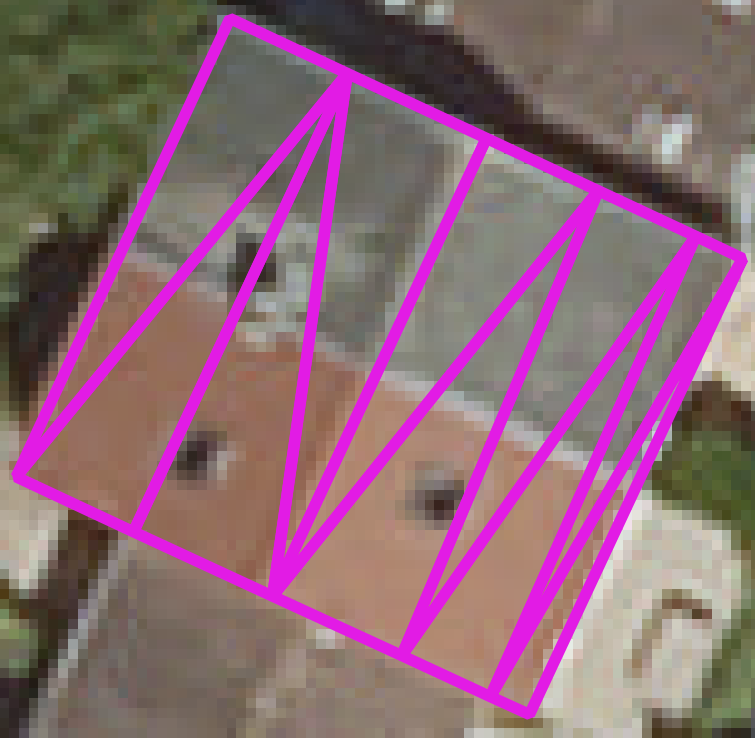
\includegraphics[height=.11\textheight]{images/Building_Errors/under_segmentation}}
                        \ffigbox[\FBwidth]{\caption{\tiny Over segmentation.}\label{fig::over_bul}}{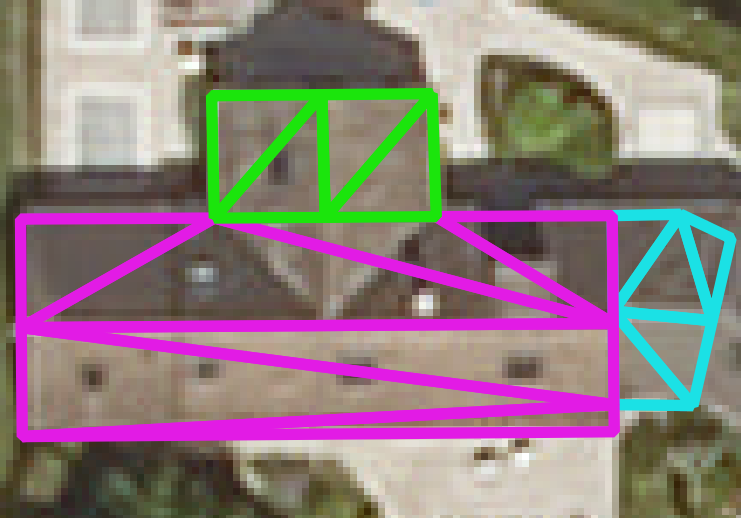
\includegraphics[height=.11\textheight]{images/Building_Errors/over_segmentation}}
                        \ffigbox[\FBwidth]{\caption{\tiny Inexact footprint.}\label{fig::footprint}}{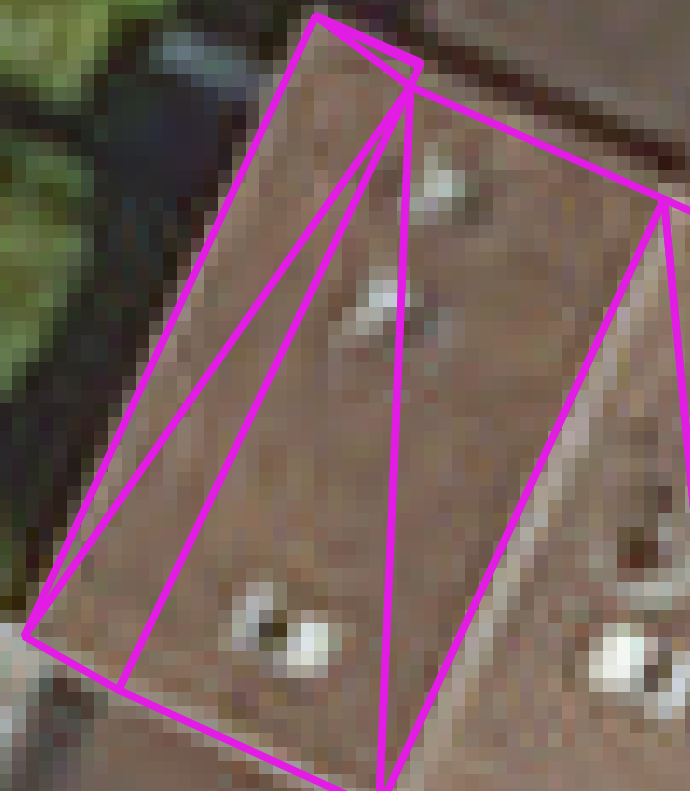
\includegraphics[height=.11\textheight]{images/Building_Errors/footprint}}
                        \ffigbox[\FBwidth]{\caption{\tiny Imprecise height.}\label{fig::too_low}}{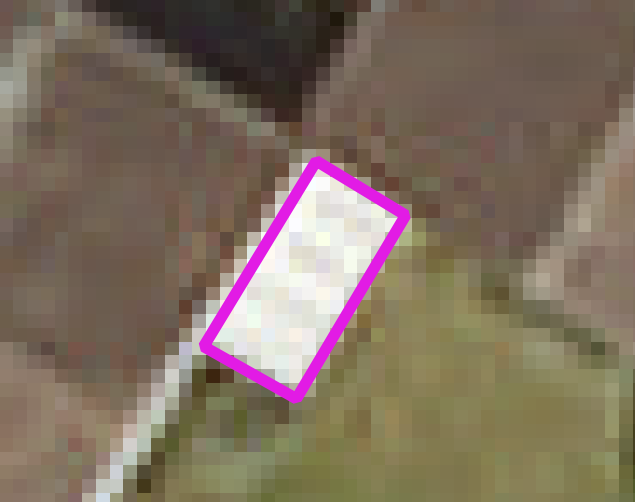
\includegraphics[height=.11\textheight]{images/Building_Errors/altimetric}}
                    \end{subfloatrow}
                }
                {
                    \captionsetup{labelfont={tiny, bf},textfont=scriptsize,justification=raggedright, labelsep=period}
                    \renewcommand{\thesubfigure}{\roman{SubFigCounter}}

                    \captionof{subfigure}{\scriptsize Building errors family samples.}\label{fig::bul_err}
                    \refstepcounter{SubFigCounter}
                    \addtocounter{figure}{-1}
                }
                \ffigbox[\FBwidth]
                {
                    \begin{subfloatrow}[4]
                        \ffigbox[\FBwidth]{\caption{\tiny Under Segmentation.}\label{fig::under_fac}}{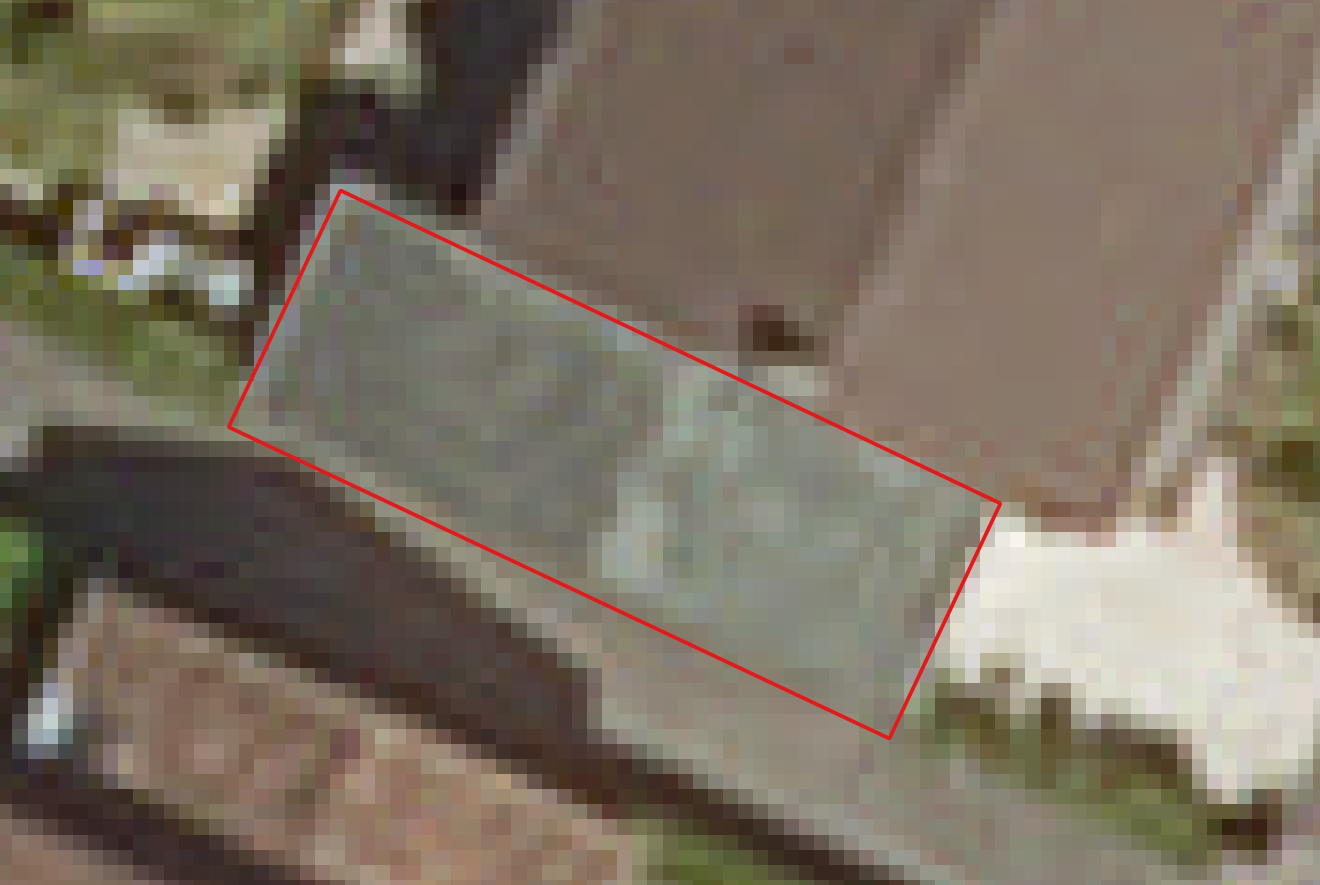
\includegraphics[height=.11\textheight]{images/Facet_Errors/under_segmentation}}
                        \ffigbox[\FBwidth]{\caption{\tiny Over segmentation.}\label{fig::over_fac}}{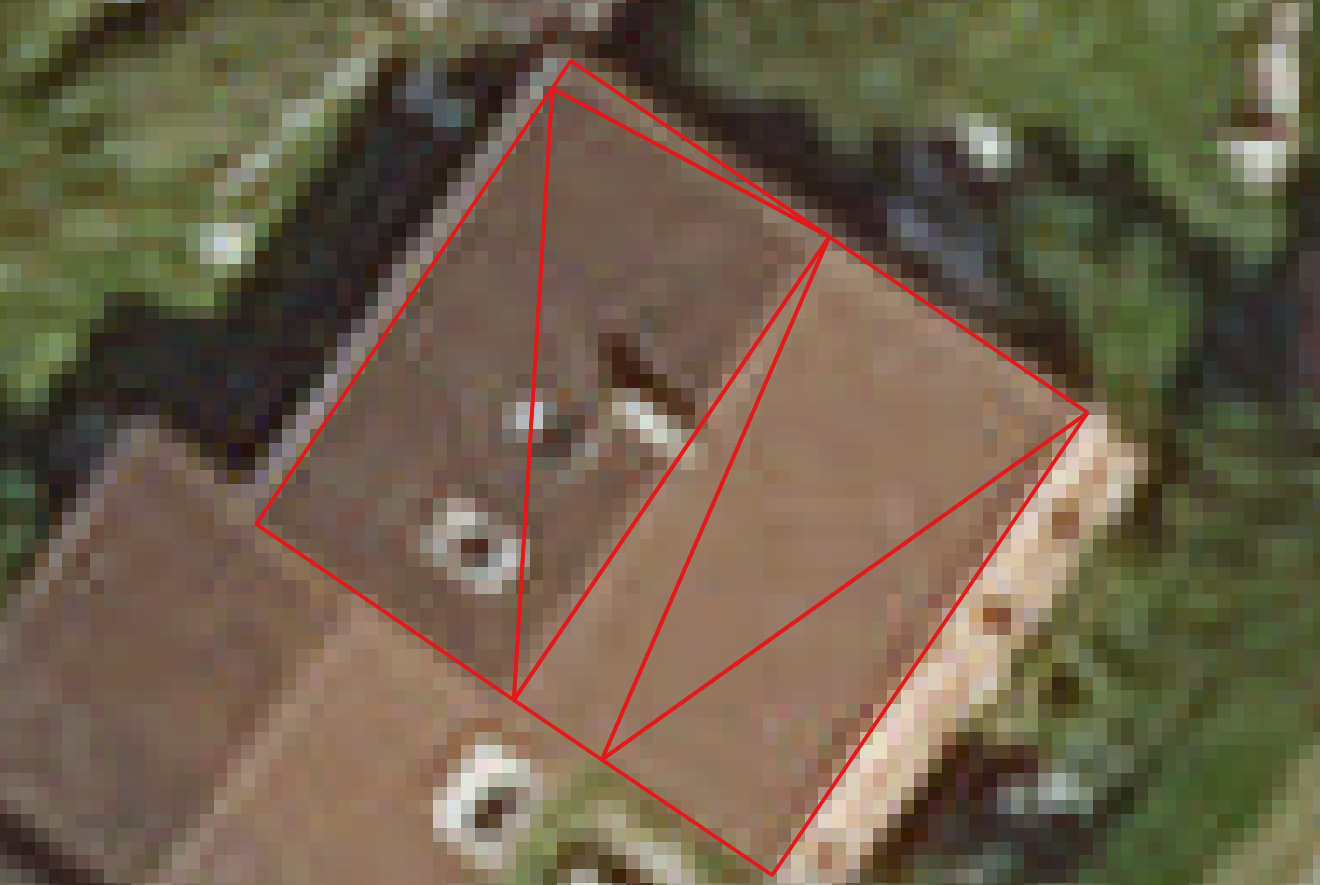
\includegraphics[height=.11\textheight]{images/Facet_Errors/over_segmentation}}
                        \ffigbox[\FBwidth]{\caption{\tiny Inexact segmentation.}\label{fig::mis}}{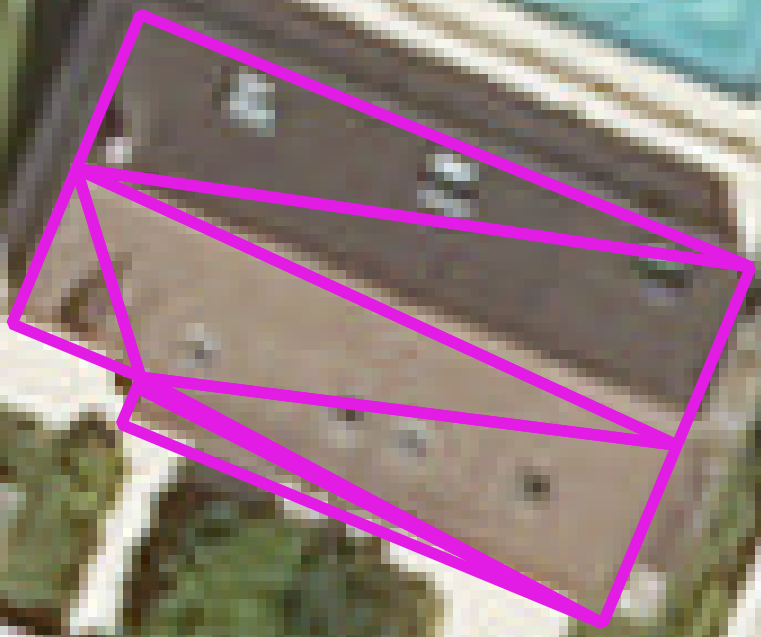
\includegraphics[height=.11\textheight]{images/Facet_Errors/mis_segmentation}}
                        \ffigbox[\FBwidth]{\caption{\tiny Imprecise slope.}\label{fig::slope}}{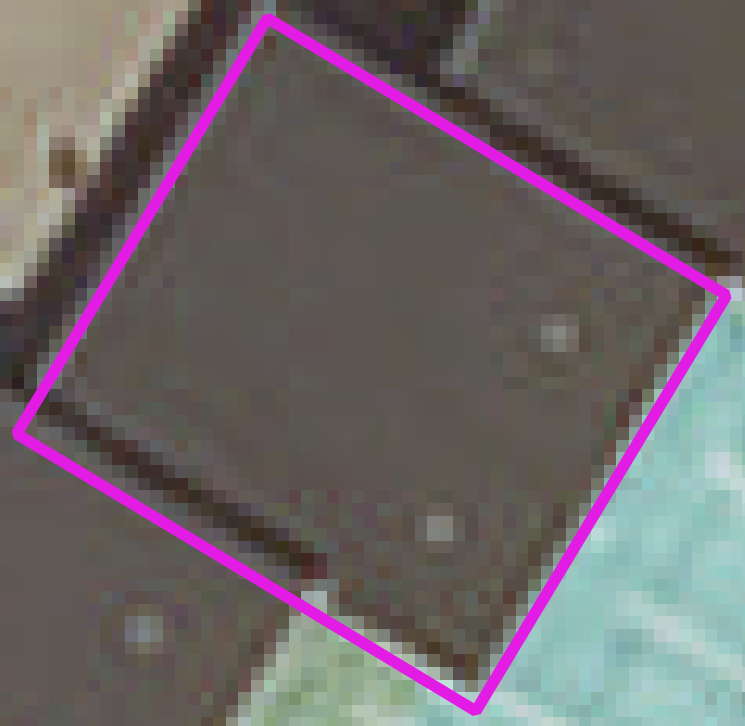
\includegraphics[height=.11\textheight]{images/Facet_Errors/slope}}
                    \end{subfloatrow}
                }
                {
                	\captionsetup{labelfont={tiny, bf},textfont=scriptsize,justification=raggedright, labelsep=period}
                    \renewcommand{\thesubfigure}{\roman{SubFigCounter}}

                    \captionof{subfigure}{\scriptsize Facet errors family samples.}\label{fig::fac_err}
                    \refstepcounter{SubFigCounter}
                    \addtocounter{figure}{-1}
                }
            }
            {
                \caption{\label{fig::samples}Error samples illustrated.}
            }
        \end{center}
    \end{figure}

    In the Figure~\ref{fig::samples}, we illustrate these errors. In (\ref{fig::under_bul}), Two building can be identified visually through the roof colors while they are grouped into one building. The contrary happens when a single building is subdivided in three parts as in (\ref{fig::over_bul}). The Inexact footprint can be detected easily when it ensues a wrongful outline as illustrated in the top right corner of (\ref{fig::footprint}). Depth information is hard to convey using images, as shown in (\ref{fig::too_low}), where the balcony, besides being detached form its building, has its height wrongly estimated due to the influence of the main building. Its also impossible to deduce the slope mis-evaluation without a depth map as is depicted in (\ref{fig::slope}). Another fidelity error can be seen in (\ref{fig::mis}), as the central edge that links the two main roof sides does not correspond to the image position. Facets can also suffer from over segmentation as both roof sides are in (\ref{fig::over_fac}). To complete the picture, (\ref{fig::under_fac}) offers a depiction of how a model roof facet can be under segmented.

\subsection{Features baseline}
In order to predict errors, models need to be described using pertinent attributes. Since there is no comparable work predicting the described errors, this work offers a baseline of features to compare with. Different from~\cite{boudet2006supervised} and~\cite{Michelin2013}, these features are kept very simple, based on depth map comparison, segment and image gradient pairing or intrinsic geometrical characteristics. The idea is to avoid heavy calculations involved in computing $3D$ lines~\cite{Michelin2013}, correlation scores~\cite{boudet2006supervised} or, in general, any greedy image matching based method. The last mentioned features are also methodologically endogamous to the $3D$ reconstruction techniques used to produce the same assessed models. In consequence, they can completely miss aspects of the reconstituted model evaluation.

The presented approach offers another degree of freedom regarding the input data to be used in model evaluation. The model itself can be of use in order to discover errors based on its geometry compared to the dataset statistics. Depth information can be added, through a \acrshort{acr::dsm}, in order to help detect defects, especially depth related ones. Last but not least, orthoimages can bring additional information critical for semantic heavy segmentation evaluation. We describe each one of these modalities, herein, in detail.

\subsubsection{Geometric features.}
The model facets set is noted $\mathsf{F}$. When two facets $(f, g) \in \mathsf{F} \times \mathsf{F}$ are adjacent --- \textit{i.e.} they share a common edge --- we write $f \sim g$. The input building model can be seen as a graph:
\begin{equation}
	\label{eq::model_graph}
	\mathsf{M} \equiv \Big(\mathsf{F}, \mathsf{E} \triangleq \big\{ (f, g) \in \mathsf{F} \times \mathsf{F} : f \sim g \big\} \Big)
\end{equation}
For each facet $f \in \mathsf{F}$, we compute its degree (\textit{i.e.} number of vertices; $d(f) \triangleq \vert\{v : v\text{ is a vertex of }f\}\vert$), its area $\mathscr{A}(f)$, the circumference $\mathscr{C}(f)$, the centroid $\mathscr{G}(f)$ and the normal $\vec{n}(f)$. We compute statistical characteristics over the building model facets, using specific families of functions $(S_p)_{p \in \mathscr{P}}$\footnote{$\mathscr{P}$ represents a parameter set. When  $\mathscr{P}=\emptyset$, we write $S$.}, like a histogram $S_{p}: l \mapsto histogram(l, p)$ or simply $S: l \mapsto \begin{bmatrix}
\max(l)& \min(l) & \bar{l} & \text{median}(l) & \sigma(l)
\end{bmatrix}$ where $\bar{l}$ (resp. $\sigma(l)$) represents the mean (\textit{resp.} the standard deviation) over a tuple $l$ and $\mathscr{P}=\emptyset$.

 For some well defined parameter $p \in \mathscr{P}$, each building $\mathsf{M}$ can be characterized by a geometric feature vector that accounts for its geometric characteristics:

\begin{equation}
	\label{eq::geom_feat}
    v_{geometric}(\mathsf{M}) = \begin{bmatrix}
    	S_p \Big(\big(d(f)\big)_{f \in \mathsf{F}}\Big)\\
    	S_p \Big(\big(\mathscr{A}(f)\big)_{f \in \mathsf{F}}\Big)\\
    	S_p \Big(\big(\mathscr{C}(f)\big)_{f \in \mathsf{F}}\Big)\\
    	S_p \Big(\big( \vert\vert \mathscr{G}(f) - \mathscr{G}(f) \vert\vert \big)_{(f,g) \in \mathsf{E}}\Big)\\
    	S_p \Big(\big( acos(\vec{n}(f), \vec{n}(g)) \big)_{(f,g) \in \mathsf{E}}\Big)
    \end{bmatrix}
\end{equation}
This type of features loses most structural information. Taking account of these implicates graph comparisons which are not genuinely simple tasks to achieve. Since the objective is to build a baseline, this approach is left for later.
\subsubsection{Altimetric features.}
For this modality, the depth information is provided as a float encoded image $dsm \in \mathbb{R}^l \otimes \mathbb{R}^w$ where $l$ and $w$ represent, respectively, the length and width of a patch containing the building projection. The model height can be inferred in function of the longitude $x$ and latitude $y$ coordinates: $h(x, y)$. The later function is quantized in the same matrix format\footnote{both top left pixels of $dsm$ and $alt$ coincide geographically and both images have the same pixel size.} as $dsm$: $alt \in \mathbb{R}^l \otimes \mathbb{R}^w$.The subtraction of these two images reveals a discrepancy map that can be exploited for the prediction (\textit{c.f.} Figure~\ref{fig::pipeline}.c). A baseline approach is proposed relying on pixel values statistics computed using previously defined functions $(S_p)_{p \in \mathscr{P}}$.
\begin{equation}
	\label{eq::alti_feat}
    v_{altimetric}(\mathsf{M}) = S_p\big( \mathrm{vec}(dsm - alt) \big)
\end{equation}
Equation~\ref{eq::alti_feat} summarizes how building altimetric features are computed. The $\mathrm{vec}$ operator represents the matrix vectorization operator. As with geometric attributes, this map loses structure representing models.
\subsubsection{Radiometric features.}
Building edges correspond to sharp discontinuities in images. The idea is to compare these edges to local gradients in order to look for inconsistencies. In an ideal setting, gradients computed at pixels $g$ of an image\footnote{containing the building} $I \in \mathbb{R}^l \otimes \mathbb{R}^w$ that intersect any segment $s$ from the building projection (\ref{fig::radio}) will almost be collinear with its normal. We qualify, using a histogram $S_p$ for a certain fixed parameter $p \in \mathscr{P}$, the distribution of the scalar product of the normalized gradient with the normal all along a segment:
\begin{equation}
	\label{eq::corr_seg}
    \mathsf{D}_p(s, I) \triangleq S_p \bigg( \Big(\frac{\nabla I(g) \cdot \vec{n}(s)}{\Vert \nabla I(g)\Vert})_{g \in I \textrm{ and } g \cap s} \Big)\bigg)
\end{equation}
Once the distribution is computed over a segment, it is compiled over all facet edges to define the distribution over projected facets. In the case of histograms, it is equivalent to summing out the previous vectors $\mathsf{D}_p(s, I)$ over segments $s$ forming the polygon projection $q(f)$ of the facet $f$. In order to take into account the variability of segment dimensions, this sum can be weighted by segment lengths.
\begin{equation}
	\label{eq::corr_fac}
	D_p(f, I) \triangleq \sum_{s \in q(f)} \Vert s \Vert \cdot \mathsf{D}_p(s, I)
\end{equation}

The same reduction can be done over all facets of a building, resulting in equation ~\ref{eq::corr_bul}. Once again, the structure of the model is lost when simply averaging over all segments.
\begin{equation}
	\label{eq::corr_bul}
	v_{radiometric}(\mathsf{M}) = D_p(\mathsf{M}, I) \triangleq \sum_{f \in \mathsf{F}} \mathscr{A}(q(f)) \cdot \mathsf{D}_p(f, I)
\end{equation}


\begin{figure}[H]
	\begin{center}
    	\floatbox{figure}{
            \begin{subfloatrow}[2]
                \ffigbox[\FBwidth]{\caption{\tiny The building projection compared to the orthoimage.}\label{fig::radio}}{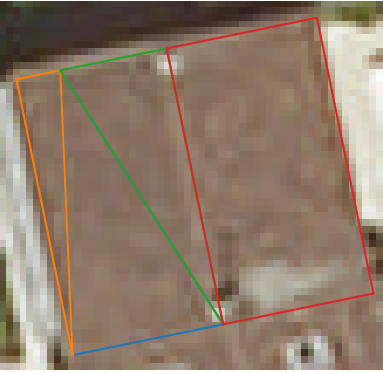
\includegraphics[width=.33\textwidth]{images/radio_vector}}
                \ffigbox[\FBwidth]{\caption{\tiny The green squares represent intersecting pixels with the red segment. The gradient in purple is compared to the segment normal in black.}\label{fig::seg_inter}}{\includestandalone[mode=buildnew, width=.33\textwidth]{radiometric_features}}
            \end{subfloatrow}
        }{
        	\caption{Radiometric features illustration.} \label{fig::radiometric}
        }
	\end{center}
\end{figure}

\subsection{Classifiers}


\section{Experiments}
\subsection{Data}
\subsection{Results}
\subsection{Discussion}
\section{Conclusion}

\bibliographystyle{splncs}
\bibliography{references}
\end{document}
